\documentclass[tikz,border=5mm]{standalone}
\usepackage{tikz}
\usetikzlibrary{arrows.meta, positioning, shapes.geometric, calc, backgrounds, fit, matrix, patterns, decorations.pathmorphing, decorations.markings, shadows}

% --- COLOR DEFINITIONS ---
\definecolor{Garnet}{HTML}{73000A}
\definecolor{CSecondaryRed}{HTML}{CC2E40}
\definecolor{CBlue}{HTML}{466A9F}
\definecolor{CDark}{HTML}{1F414D}
\definecolor{COlive}{HTML}{65780B}
\definecolor{CLime}{HTML}{CED318}
\definecolor{CGold}{HTML}{A49137}
\definecolor{CGrayLight}{HTML}{E5E5E5}
\definecolor{CGrayDark}{HTML}{555555}
\definecolor{CWhite}{HTML}{FFFFFF}

\begin{document}

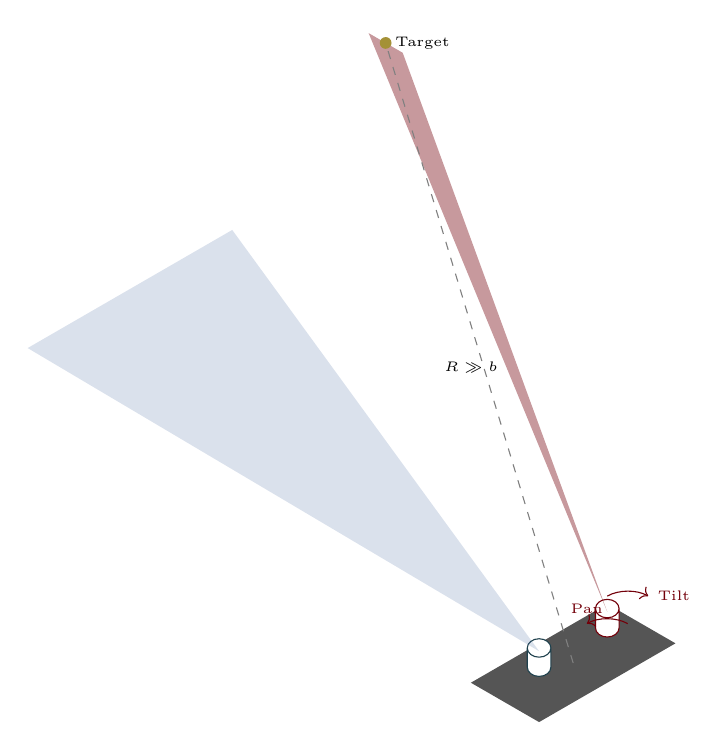
\begin{tikzpicture}[x={(0.866cm,0.5cm)}, y={(-0.866cm,0.5cm)}, z={(0cm,1cm)}]
    % Platform
    \fill[CGrayDark] (-1, -0.5, 0) -- (1, -0.5, 0) -- (1, 0.5, 0) -- (-1, 0.5, 0) -- cycle;
    
    % Cam 1 (Fixed) at (-0.5, 0, 0)
    \node[cylinder, draw=CDark, fill=CWhite, rotate=90, minimum height=0.3cm, minimum width=0.3cm] at (-0.5, 0, 0.2) {};
    
    % Cam 2 (PTZ) at (0.5, 0, 0)
    \node[cylinder, draw=Garnet, fill=CWhite, rotate=90, minimum height=0.3cm, minimum width=0.3cm] (Cam2) at (0.5, 0, 0.2) {};
    
    % 3D Spherical Coordinate Arrows for Cam 2
    \draw[->, Garnet] (0.5, 0, 0.6) arc (90:0:0.3) node[right, font=\tiny] {Tilt};
    \draw[->, Garnet] (0.8, 0, 0.1) arc (0:90:0.3) node[above, font=\tiny] {Pan};
    
    % Projection Beams
    % Fixed Beam
    \fill[CBlue, opacity=0.2] (-0.5, 0, 0.4) -- (-2, 6, 2) -- (1, 6, 2) -- cycle;
    
    % Zoom Beam (Narrow, Directed Up)
    \fill[Garnet, opacity=0.4] (0.5, 0, 0.4) -- (3, 6, 3.5) -- (3.5, 6, 3) -- cycle;
    
    % Dashed line to distant target
    \draw[dashed, gray] (0, 0, 0) -- (3.25, 6, 3.25);
    \node[font=\tiny] at (1.5, 3, 1.5) {$R \gg b$};
    
    % Target
    \node[circle, fill=CGold, inner sep=1.5pt] at (3.25, 6, 3.25) {};
    \node[right, font=\tiny] at (3.25, 6, 3.25) {Target};
    
\end{tikzpicture}

\end{document}
